\documentclass{beamer}

\mode<presentation>
\usetheme{Warsaw}
\usefonttheme[onlylarge]{structurebold}
\usecolortheme[RGB={0,120,90}]{structure}
\setbeamerfont{frametitle}{size=\normalsize,series=\bfseries}
\setbeamertemplate{navigation symbols}{}
\setbeamertemplate{background canvas}{
\includegraphics[width=\paperwidth,height=\paperheight]{images/pgbr.eps}}
\setbeamercovered{transparent=95}
\setbeamertemplate{blocks}[rounded][shadow=true]



\usepackage[brazil]{babel}
\usepackage[utf8]{inputenc}
\usepackage{times}
\usepackage[T1]{fontenc}

\usepackage{tikz}
\usetikzlibrary{arrows}
\tikzstyle{block}=[draw opacity=0.7,line width=1.4cm]

\title[Pgbouncer, plproxy, skytools]
{%
   PostgreSQL para um bilhão de usuários%
}

\author[Fernando Ike de Oliveira]
{
   \textcolor{red!50!black}{Fernando Ike de Oliveira}
}

\institute[B2BR]
{
 \textcolor{green!30!black}{B2BR - Grupo TBA}
}

\date[Short Occasion]
{Setembro de 2008 / PGCon-BR 2008}
\logo{
\includegraphics[scale=0.1]{images/b2br}}

\begin{document}
\begin{frame}
\titlepage
\end{frame}




\begin{frame}
  \frametitle{\textbf{Breve história...}}
    \begin{itemize}
      \item 2004 libera um conjunto de ferramentas para 
          replicação, balanceamento de carga e alta-disponibilidade 
	  para PostgreSQL.
      \item Essas ferramentas são conhecidas como PL/Proxy, 
          PgBouncer, Skytools.
      \item A licença é BSD.
      \item Instalação à partir do código-fonte ou pacotes *.deb *.rpm.
      \item Oficialmente o Debian, Fedora tem pacotes binários.
      \end{itemize}

\end{frame}

\begin{frame}
  \frametitle{\textbf{PL/Proxy}}
    \begin{itemize}
      \item PL/Proxy é uma linguagem usada para chamadas remotas
        e particionamento de banco de dados usando hash dos dados.
      \item PL/Proxy permite criar funções de proxy usando hash
        para especificar destino (base de dados alvo). 
      \item PL/Proxy é comparável à um roteador de rede que encaminha a 
        expressão SQL para o instância correta.
  \end{itemize}

\end{frame}

\begin{frame}
  \frametitle{\textbf{PL/Proxy}}
  \framesubtitle{Princípio de funcionamento PL/Proxy}
  \begin{block}{Exemplo}
    \small{\textit{"SELECT (hashtext('pgcon1'))\%3"} \hspace{0.1cm}\textbf{=}  \hspace{0.1cm} \alert{0}} \\
    \small{\textit{"SELECT (hashtext('pgcon2'))\%3"} \hspace{0.1cm}\textbf{=}  \hspace{0.1cm} \alert{-1}} \\
    \small{\textit{"SELECT (hashtext('pgcon3'))\%3"} \hspace{0.1cm}\textbf{=}  \hspace{0.1cm} \alert{-2}} \\
    \small{\textit{"SELECT (hashtext('pgcon4'))\%3"} \hspace{0.1cm}\textbf{=}  \hspace{0.1cm} \alert{0}} \\
    \small{\textit{"SELECT (hashtext('pgcon5'))\%3"} \hspace{0.1cm}\textbf{=}  \hspace{0.1cm} \alert{0}} \\ 
    \small{\textit{"SELECT (hashtext('pgcon6'))\%3"} \hspace{0.1cm}\textbf{=}  \hspace{0.1cm} \alert{2}} \\ 
    \small{\textit{"SELECT (hashtext('pgcon7'))\%3"} \hspace{0.1cm}\textbf{=}  \hspace{0.1cm} \alert{-1}} \\ 
    \small{\textit{"SELECT (hashtext('pgcon8'))\%3"} \hspace{0.1cm}\textbf{=}  \hspace{0.1cm} \alert{0}} \\
    \small{\textit{"SELECT (hashtext('pgcon9'))\%3"} \hspace{0.1cm}\textbf{=}  \hspace{0.1cm} \alert{0}} \\
    \small{\textit{"SELECT (hashtext('pgcon10'))\%3"} \hspace{0.1cm}\textbf{=} \hspace{0.1cm} \alert{0}} \\
  \end{block}


\end{frame}

\begin{frame}
  \frametitle{\textbf{PL/Proxy}}
  \framesubtitle{idéias básicas possíveis}
    \begin{block}{ }
    \begin{itemize}
      \item Como um barramento, para todos as servidores PostgreSQL
      \item Tabelas
      \item Particionamento usando funções de Proxy 
    \end{itemize}
    \end{block}
\end{frame}

\begin{frame}
    \frametitle{\textbf{PL/Proxy}}
    \framesubtitle{Problema}
  \begin{center}
     \pgfputat{\pgfxy(-113,-100)}{\pgfimage[width=\paperwidth,height=\paperheight]{images/cenario_ori.eps}}
      \par
  \end{center}


\end{frame}

\begin{frame}
    \frametitle{\textbf{PL/Proxy}}
    \framesubtitle{Princípio do Proxy}
  \begin{center}
     \pgfputat{\pgfxy(-113,-100)}{\pgfimage[width=\paperwidth,height=\paperheight]{images/proxy.eps}}
      \par
  \end{center}


\end{frame}


\begin{frame}
    \frametitle{\textbf{PL/Proxy}}
    \framesubtitle{Particionamento de dados}
  \begin{center}
%     \pgfputat{\pgfxy(-113,-100)}{\pgfimage{images/part_db_user.eps}}
     \pgfputat{\pgfxy(-113,-100)}{\pgfimage[width=\paperwidth,height=\paperheight]{images/part_db_user.eps}}
      \par
  \end{center}


\end{frame}

\begin{frame}
    \frametitle{\textbf{PgBouncer}}
    \framesubtitle{Um serviço de pool para o PostgreSQL}
      \begin{itemize}
      \item Baixo consumo de recurso (2k por conexão)
      \item Suporta reconfiguração sem reiniciar o serviço
      \item Suporta reinício/atualização sem derrubar a conexão cliente
      \item Suporta o protocolo v3 ou superior, somente => \alert{7.4}
      \item O Parse \alert{SQL} nao eh muito rápido e consome pouco tempo de cpu
      \item Tem uma interface console de gerenciamento 
      \item Tem estrutura sua (própria) estrutura de autenticação mas similar ao arquivo similar ao arquivo de senha pg\_pwd do PostgreSQL.
      \item Permite autenticação do tipo: trust, texto plano, crypt, md5.
      \end{itemize}

\end{frame}

\begin{frame}
    \frametitle{\textbf{PgBouncer}}
    \framesubtitle{Modos de pool}
        \begin{itemize}
	 \item Sessão (session)
         \item Transação (transaction)
         \item Instrução (statement)
	\end{itemize}
\end{frame}

\begin{frame}
    \frametitle{\textbf{PgBouncer}}
    \framesubtitle{Sessão}
      \begin{itemize}
        \item Quando um cliente conecta, o PgBouncer retira uma conexão do pool e entrega para a aplicação
	\item Ao o cliente desconectar, o PgBouncer re-aloca a conexão para o pool. geralmente essa configuração é recomendada para aplicações legadas(Por não usarem de forma eficiente o pool)
      \end{itemize}


\end{frame}

\begin{frame}
    \frametitle{\textbf{PgBouncer}}
    \framesubtitle{Transação}
      \begin{itemize}
        \item Servidor mantém para o cliente a conexão somente durante a transação. Quando PgBouncer notifica que transação acabou, o servidor devolve a conexão para o pool. 
	\item Essa opção não deve ser usada com servidor de aplicações que gerenciam pool (Jboss, por exemplo)
      \end{itemize}
\end{frame}

\begin{frame}
    \frametitle{\textbf{PgBouncer}}
    \framesubtitle{Instrução (Statement)}
      \begin{itemize}
        \item Este é o modo usado usado com o PL/Proxy. Por ser mais agressivo, ele retornar o conexão para opool depois que a consulta termina.
	\item Transações muito longas com múltiplos Statements são desabilitados neste modo. 
      \end{itemize}

\end{frame}


\begin{frame}
    \frametitle{\textbf{Skytools}}
    \framesubtitle{O que é?}
      \begin{itemize}
        \item Skytools são um conjunto de scripts para gerenciar cluster de servidores PostgreSQL.
	\item Desenvolvido em C e Python
	\item Permitem usar para replicação assíncrona
	\item Permitem replicar dados particionados nos servidores "slave(s)"
	\item Possível extender usando as API do PgQ

      \end{itemize}


\end{frame}


\begin{frame}
    \frametitle{\textbf{Skytools}}
    \framesubtitle{Basicamente...}
      \begin{itemize}
        \item Centralização de log gerenciamento de exceções.
	\item Gerenciamento de conexões ao banco de dados
	\item Gerenciamento de configuração
	\item Gerenciamento de scrips...
      \end{itemize}
\end{frame}


\begin{frame}
    \frametitle{\textbf{Skytools}}
    \framesubtitle{Conteúdo}
      \begin{itemize}
      \item londiste 
      \item walmgr 
      \item serial\_consumer
      \item queue\_mover 
      \item queue\_splitter
      \item table\_dispatcher
      \item cube\_dispatcher
      \end{itemize}
\end{frame}


\begin{frame}
    \frametitle{\textbf{Skytools}}
    \framesubtitle{Londsite é...}
      \begin{itemize}
        \item ... um sistema de replicação
        \item ... Master/Slave(s) como tipo de replicação
        \item ... de replicação é assíncrona
        \item ... baseada fortemente nas idéias do no Slony-1.
        \item ... um replicador baseado em gatilhos
      \end{itemize}


\end{frame}

\begin{frame}
    \frametitle{\textbf{Skytools}}
    \framesubtitle{Walmgr é...}
      \begin{itemize}
        \item ... uma ferramenta para gerenciar replicação por WAL
        \item ... similar ao pg\_standby (contrib)
        \item ... possível gerenciar replicação baseada em PITR (Warm Standby).
        \item ... escrito em python
        \item ... uma ferramenta de replicação que usa túnel SSH.
      \end{itemize}
\end{frame}

\begin{frame}
    \frametitle{\textbf{Skytools}}
    \framesubtitle{queue\_mover e queue\_splitter}
       \begin{block}{Ambos}
         \begin{itemize}
	   \item Usa o PgQ como transporte dos dados
	   \item Move/copia os dados para os servidores Slave
	   \item Move/copia os dados em lote(batch)
	   \item O processamento é/são nos slave(s)
	 \end{itemize}

       \end{block}
       
       \begin{block}{queue\_mover}
         \begin{itemize}
	   \item Usado para mover/copia os dados para OLTP, Web
 	 \end{itemize}
       \end{block}

       \begin{block}{queue\_splitter}
          \begin{itemize}
	    \item Usado para BI
	 \end{itemize}

        \end{block}
      
\end{frame}


\begin{frame}
    \frametitle{\textbf{Skytools}}
    \framesubtitle{cube\_dispacher e table\_dispacher}
      \begin{block}{Ambos}
         \begin{itemize}
           \item Ferramentas para replicar dados em tabelas particionadas.
	   \item Usados para preparar os dados para outros servidores
         \end{itemize}
       \end{block}

      \begin{block}{cube\_dispacher}
         \begin{itemize}
	   \item Prepara os dados para banco de dados do tipo BI, OLAP, Cubo...
	   \item Não tem suporte para operações de remoção de registro
	   \item Caso haja duas versões do mesmo registro, ele irá enviar somente a última versão.
	 \end{itemize}
      \end{block}

      \begin{block}{table\_dispacher}
        \begin{itemize}
	  \item script para configuraro particionamento de uma ou mais tabela.
	  \item possibilita particionar uma tabela por mês, por exemplo.
	\end{itemize}
      \end{block}
\end{frame}



\begin{frame}
    \frametitle{\textbf{Exemplo 1}}
     \begin{center}
       \pgfputat{\pgfxy(-113,-100)}{\pgfimage[width=\paperwidth,height=\paperheight]{images/scalling.eps}}
       \par
      \end{center}


\end{frame}

\begin{frame}
    \frametitle{\textbf{Exemplo 2}}
     \begin{center}
       \pgfputat{\pgfxy(-113,-100)}{\pgfimage[width=\paperwidth,height=\paperheight]{images/plproxy.eps}}
       \par
      \end{center}


\end{frame}


\begin{frame}
    \frametitle{\textbf{Dúvidas}}

    \begin{block}{Links e Listas de discussão:}
        \begin{itemize}
            \item {\textbf{\tiny \url{https://developer.skype.com/SkypeGarage/DbProjects/SkypePostgresqlWhitepaper}}}
            \item {\textbf{\tiny \url{https://developer.skype.com/SkypeGarage/DbProjects/PlProxy}}}
            \item {\textbf{\tiny \url{http://pgfoundry.org/mailman/listinfo/plproxy-users}}}
            \item {\textbf{\tiny \url{https://developer.skype.com/SkypeGarage/DbProjects/PgBouncer}}}
            \item {\textbf{\tiny \url{http://pgfoundry.org/mailman/listinfo/pgbouncer-general}}}
            \item {\textbf{\tiny \url{https://developer.skype.com/SkypeGarage/DbProjects/SkyTools}}}
            \item {\textbf{\tiny \url{http://pgfoundry.org/mailman/listinfo/skytools-users}}}
            \item {\textbf{\tiny \url{http://joaocosme.wordpress.com/2008/07/03/comecando-com-o-plproxy/}}}
        \end{itemize}
    \end{block}

\end{frame}







\begin{frame}
    \frametitle{\textbf{Conclusão}}
    \begin{block}{Contatos:}
        \begin{itemize}
            \item {\texttt{fernando.ike@b2br.com.br}}
            \item {\texttt{fernando.ike@gmail.com}}
            \item {\textit{\url{ http://www.midstorm.org/~fike/weblog}}}
        \end{itemize}
    \end{block}

    \begin{block}{PGCon Brasil 2008}
        \begin{itemize}
            \item {\textit{\url{http://pgcon.postgresql.org.br}}} \\
            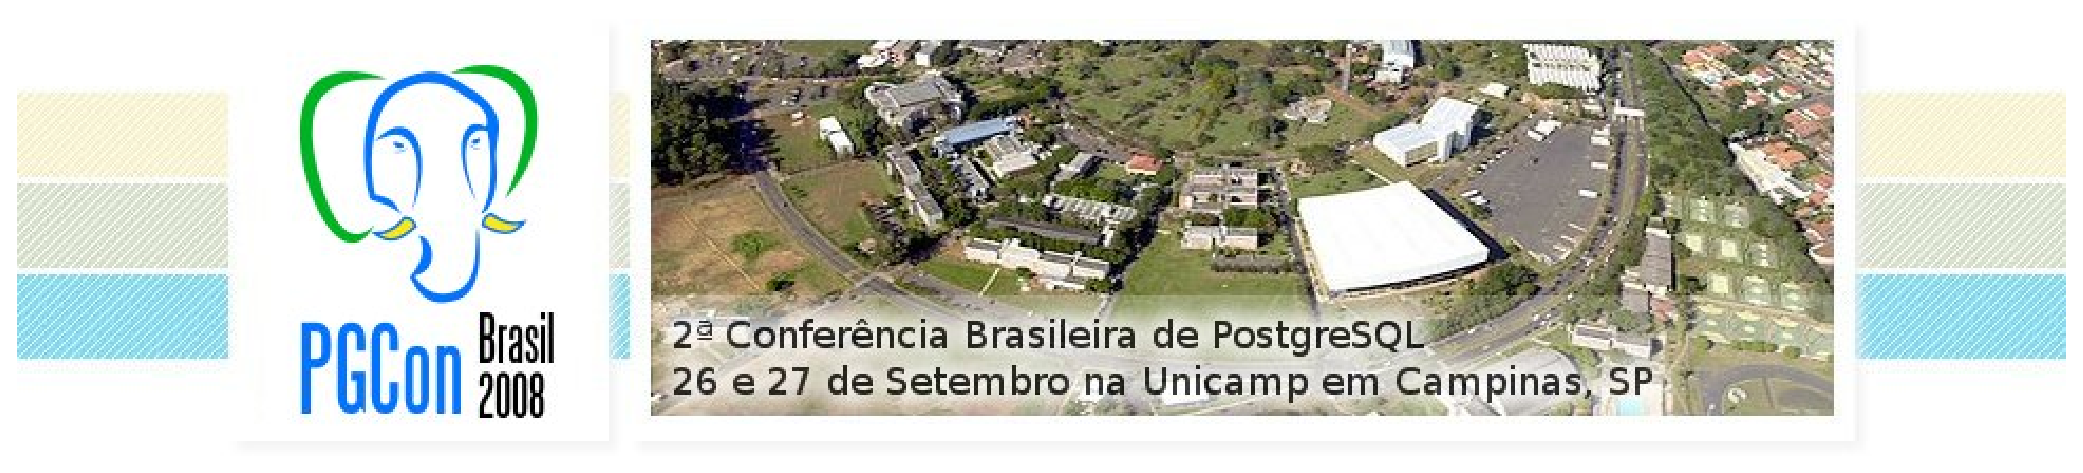
\includegraphics[scale=0.2]{images/pgconbr.eps}
        \end{itemize}
    \end{block}

    \begin{block}{Imagens}
        \begin{itemize}
	  \item Joao Comes {\textit{\url{ http://joaocosme.wordpress.com}}}
        \end{itemize}  
    \end{block}


\end{frame}


\end{document}
